%   Copyright (C) 2014  School of Information Sciences, Manipal



\newcommand{\projecttitle}{Boot-Time Optimization for Android on Intel Atom Architecture}
\newcommand{\projectauthors}{\normalsize Aurabindo J (141021001)}

\documentclass{mainreport}
\linespread{1.5}
\usepackage{hyperref}
\usepackage{makeidx}
\usepackage{multirow}
\usepackage{nomencl}
\usepackage{pdfpages}
\usepackage{subcaption}
\usepackage{tabularx}
\usepackage{listings}
\usepackage{color}
\usepackage{upquote}
%\usepackage{biblatex}

\definecolor{dkgreen}{rgb}{0,0.6,0}
\definecolor{gray}{rgb}{0.5,0.5,0.5}
\definecolor{mauve}{rgb}{0.58,0,0.82}


\lstset{frame=tb,
  aboveskip=3mm,
  belowskip=3mm,
  showstringspaces=false,
  columns=flexible,
  basicstyle={\small\ttfamily},
  numbers=none,
  numberstyle=\tiny\color{gray},
  keywordstyle=\color{blue},
  commentstyle=\color{dkgreen},
  stringstyle=\color{mauve},
  breaklines=true,
  breakatwhitespace=true
  tabsize=3
}

%\usepackage{tocloft}


\newcommand{\tab}{\hspace*{2em}}
% for removing dots

\makeatletter
\renewcommand{\@dotsep}{10000} 
\makeatother

\renewcommand{\figurename}{Fig.}


\begin{document}

\maketitle
\makecertificate

\parindent 10mm
%\newgeometry{bottom=2.5cm,top=2.5cm}
\chapter*{Acknowledgment}\label{ack}\addcontentsline{toc}{chapter}{Acknowledgment}
{\label{ack} 

%\paragraph*{•}
\hspace{6mm} This project itself is an acknowledgment to the inspiration, drive and technical
assistance contributed by many individuals. I would like to express my heartfelt thanks to my project guide {\bf Dr. S. Arockiaraj}. We also like to express our gratitude towards {\bf Dr. B. Dinesh Rao}.
%\paragraph*{•}
I would like to thank {\bf School of Information Science}, in particular, for providing us with an ample environment and
infrastructure required to carry out this project. I take this opportunity to thank
the {\bf Dr. Harishchandra Hebbar}, as the director of the School of Information Sciences, for the inspiration and support rendered.

%\paragraph*{•}
I extend my heartfelt thanks to my parents, friends and well wishers for their support and timely help. Above all I thank the Almighty for His blessing and providing mercies at all stages of my work. \\[2cm]




\noindent Manipal \hfill Project Members

\noindent \today \hfill School of Information Sciences

 \hfill Manipal





}

\chapter*{Abstract}\label{Abstract}\addcontentsline{toc}{chapter}{Abstract}

{
\label{Abstract}



%\paragraph*{•}
\hspace{6mm} Modern encryption systems are very advanced and are practically impossible to break them by using a brute force attack in a time bound manner. This project aims at exploiting the validity of the message data and then encrypt it using a key. The key length depends on the validity duration of the data. Data that is important and has longer validity will be encrypted using a longer key, and the data which has shorter validity is encrypted using a shorter key. Point being that at any given point, the time taken to decipher the content is greater than the validity period of the data. If it will be invalid for an attacker after say, 1 minute, then encoding that data with a very large key is a penalty as the attacker cannot break it in that short time. So we use a smaller key length to encrypt it. The advantage is better encryption throughput without compromising security.
%\end{center}
}

%generate table of contents
\tableofcontents

%\chapter*{List of Symbols}\label{symbol}\addcontentsline{toc}{chapter}{List of Symbols}
%\listofsymbols

%\input{symbol}

%\input{fig}

\addcontentsline{toc}{chapter}{List of Figures}



\listoffigures
%\listoftables
\addtocontents{lof}{\textbf{No.}\hspace{8 mm}\textbf{Figure}~\hfill\textbf{Page}\par}
%\newpage


\chapter*{List of Abbreviations}\label{abbrv}\addcontentsline{toc}{chapter}{List of Abbreviations}




%Add your abbreviations here as follows
%\nomenclatue{Abbr}{Abbreviation}
%Example:
%\makenomenclature
\begin{center}
\label{abbrv}
\begin{tabular}{r l}
	TTYL & Talk To You Later \\
	AFAIK & As Far As I Know \\
	IMHO & In My Humble Opinion \\
	IMO & In My Opinion (not so humble)\\
	ROFL & Rolling On The Floor and Laughing
\end{tabular}
\end{center}


\newpage



%\chapter*{Report}\label{report}\addcontentsline{toc}{chapter}{Report}

\pagenumbering{arabic}





\section{Introduction}
\label{report}


\hspace{8mm} 

\noindent Mobile devices are the one of the most competitive consumer technology equipment market.
Manufacturers come up with improved or advanced versions of their product quite sooner that
people expect. With the demand from the market for more of performance, features, battery
life, etc the need to optimizing existing products also arise. Hence optimization of boot time
for Android devices are quite relevant.

We will look into the overview of Android booting sequence from all levels. Then we will look
deeply into available tools to evaluate the boot time. Various profiling tools which help understand
the booting process in detail will also be covered in detail. Finally we will look at the techniques
and procedures which will help in reducing the boot time. The optimizing effort will be focused on the
linux kernel and bootloader.

\subsection{About Android}

Android is an open source mobile OS currently developed by Google, based on the Linux kernel and designed
primarily for touchscreen mobile devices such as smartphones and tablets. Initially developed
by Android, Inc., which Google bought in 2005. Android was unveiled in 2007, along with the
founding of the Open Handset Alliance – a consortium of hardware, software, and telecommunication
companies devoted to advancing open standards for mobile devices. However, most Android devices
ultimately ship with a combination of open source and proprietary software, including proprietary
software required for accessing Google services.


Linux kernel is the core part of the Android OS. The version of the linux kernel used in Android is
based on one of the Linux kernel's LTS branches. Android's variant of the Linux kernel has further
architectural changes that are implemented by Google outside the typical Linux kernel development
cycle, such as the inclusion of components like Binder, ashmem, pmem, logger, wakelocks,
and different out-of-memory (OOM) handling.

\subsubsection {Hardware}

The main hardware platform for Android is the ARM architecture (ARMv7 and ARMv8-A architectures),
with x86 and MIPS architectures also officially supported in later versions of Android.
Since Android 5.0 "Lollipop", 64-bit variants of all platforms are supported in
addition to the 32-bit variants.

Intel has its processors specifically made for low power devices, which run Android.
This architecture is known as Intel Atom. It is a SoC which offers good performance with
reduced power consumption compared to a full fledged desktop processors known under
the series Intel Core.

\subsubsection{Software Stack}

On top of the Linux kernel, there are the middleware, libraries and APIs written in C,
and application software running on an application framework which includes
Java-compatible libraries based on Apache Harmony. Development of the Linux kernel
continues independently of other Android's source code bases.

\begin{figure}[h]
  \centering
    \centering
    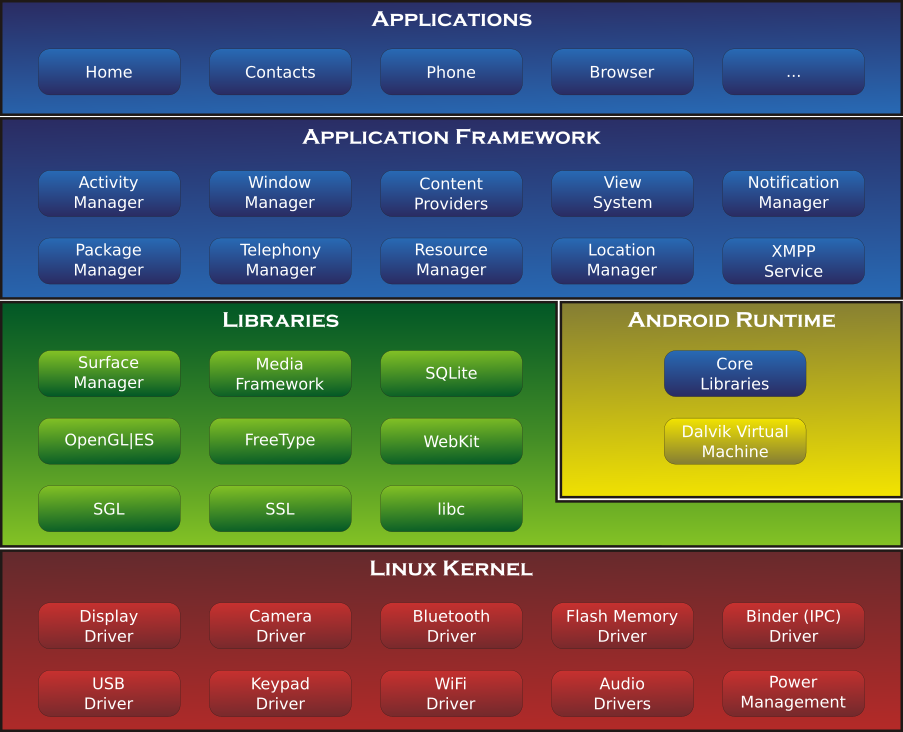
\includegraphics[scale=0.6]{android_arch.png}
    \caption{Android Software Architecture}
    \label{fig:android_arch}
\end{figure}

%\begin{figure}[h!]
%  \centering
%    	\includegraphics[scale=0.5]{scada_architecture.png}
%	\caption{Architecure of a typical power SCADA system}
%	\label{scada_arch} %the label was cycle here



%\begin{figure}[h]
%  \centering
%  \begin{subfigure}[b]{1\textwidth}
%    \centering
%    \includegraphics[scale=0.4]{digraph_simple.png}
%    \caption{relation digraph of the simplified system}
%    \label{fig:digraph_simple}
%  \end{subfigure}
  
%  \begin{subfigure}[b]{1\textwidth}
%    \centering
%    \includegraphics[scale=0.4]{digraph_virtual.png}
%    \caption{Representation of the digraph with virtual nodes}
%    \label{fig:digraph_virtual}
%  \end{subfigure}
  
%\end{figure}



%\chapter*{Datasheets}\label{datasheet}\addcontentsline{toc}{chapter}{Datasheets}

%{\label{nexys3}\includepdf[pages={-}]{Nexys3_rm.pdf} 
%{\label{nexys3}\includepdf[pages={1-1,8-10,11-14,18-20}]{Nexys3_rm.pdf} 
%{\label{nexys3}\includepdf[pages={1-1}]{spartan6.pdf} 

\nocite{*}
\bibliographystyle{plain}
\bibliography{master}

\end{document}
